\documentclass[letterpaper]{article}

% PACKAGES
\usepackage[utf8]{inputenc}
% Your extra packages here
%
\usepackage{graphicx}
\usepackage[colorlinks=true, citecolor=black, linkcolor=black, urlcolor=blue]{hyperref}
\usepackage{array,multirow}
\usepackage{tabularx}
\usepackage{hhline}
\usepackage{makecell}
\usepackage[obeyFinal,colorinlistoftodos]{todonotes}
\usepackage{courier}

\title{Evolutionary Origins of Transformation via Natural Competence}
\author{Rosangela Canino-Koning$^{1,2,3}$, Michael J. Wiser$^{2,3}$, Charles Ofria$^{1,2,3}$}

\begin{document}
\maketitle
~\\
$^{1}$Department of Computer Science and Engineering, Michigan State University, East Lansing, MI, USA \\
$^{2}$BEACON Center for the Study of Evolution in Action, Michigan State University, East Lansing, MI, USA \\
$^{3}$Ecology, Evolutionary Biology, and Behavior, Michigan State University, East Lansing, MI, USA\\

\begin{abstract}
\todo[inline]{ABSTRACT}
Abstract!
\end{abstract}

\todototoc
\listoftodos

\section{Introduction}

%=HGT umbrella term
Horizontal Gene Transfer (HGT) is a broad term for the non-reproductive transfer of genetic material between organisms. Organisms may uptake genes directly from the environment (transformation via natural competence~\cite{chen_dna_2004}), or else receive them via bacterial conjugation~\cite{lederberg_gene_1946} or viral infection (transduction~\cite{zinder_genetic_1952,lennox_transduction_1955}). In the case of transformation, the fragments may either be decomposed inside the recipient cell for their nutrients, or recombined into their genomes. 

%=HGT profound impact
HGT has had a profound impact on the evolutionary history of both prokaryotes and eukaryotes, with one study showing approximately 81\% of genes in the sample "being involved in HGT at some point in their history"~\cite{dagan_modular_2008}. For example, HGT appears to be the primary mechanism by which antibiotic resistance is conferred~\cite{davies_origins_1997,martinez_antibiotics_2008} since most antibiotics are sourced from the environment, and the organisms that develop them are themselves resistant to the compounds.
However, the origins and evolution of HGT mechanisms remain unclear. 

\subsection{Origins of Horizontal Gene Transfer in nature}
%=natural competence in prokaryotes and why HGT happens
In prokaryotes, ``transformation'' is an HGT mechanism by which organisms spontaneously uptake the DNA of dead organisms in the environment. Competent organisms benefit in several ways. 1) DNA is composed of a 5-carbon sugar, a phosphate, and nitrogenous bases, materials that are useful for DNA synthesis and repair. 2) The organisms may also benefit from taking up gene fragments that confer new adaptive functionality into the genome~\cite{vos_why_2009}. However, it is unclear whether the origins of transformation functions were developed solely in order to obtain nutrients (the Grazing Hypothesis), or if the acquisition of new functionality was selected for as well. While grazing for gene fragments as nutrients certainly conveys an advantage, the possibility of integrating these gene fragments is likely to be deleterious to organisms more often than it is beneficial~\cite{redfield_evolution_1997}. For example, since the DNA would be originating from dead organisms, DNA fragments may be of low quality, and recombine deleterious mutations, or even remove competence altogether~\cite{redfield_evolution_1997}. Alternately, errors in homologous recombination may apply fragments to random locations in the genome.    

Although advances in molecular biology are allowing researchers to investigate the mechanisms of HGT and even reconstruct specific inferred cases of HGT (as reviewed in Bock 2015~\cite{bock_witnessing_2015}), the processes themselves are ancient and nearly ubiquitous~\cite{soucy_horizontal_2015}. This very ancientness makes studying the early evolution of HGT in physical organisms exceedingly challenging, as we lack easily tractable systems that differ only in whether or not HGT exists within them. Therefore, empirical studies in natural systems remain exceedingly rare.

%=statement of hypotheses - grazing CE elevates HGT
\todo[inline]{define what we mean by a harsh changing environment}
In order to test the Grazing Hypothesis of the origin of HGT, and to address the question of whether there are circumstances where gene fragment integration may be beneficial, subjected populations of evolving digital organisms to a harsh changing environment,
% MJW: For the dissertation, this is probably fine, since you have a chapter about changing environments immediately before this one. For a paper, we'll need to define what we mean by a harsh changing environment -- it's pretty standard nomenclature in the field of people who look at changing environments, but not all readers will know it.
where there is a strong selective pressure to quickly switch phenotype. We supplied organisms with an instruction that performs Horizontal Gene Transfer (\texttt{HGT-Uptake}). That is, the instruction triggers uptake of a genetic fragment from the environment, and there is a probability that, rather than metabolizing the fragment for a bonus to execution speed, the fragment will instead be homologously recombined into the organism's genome. We show that in harsh changing environments, without any kind of bonus, organisms increase use of HGT as compared to execution in a static environment.

\section{Methods}

In this chapter, we use Avida to test hypotheses about the origins of Horizontal Gene Transfer. 

\subsection{HGT in Avida}
%=HGT triggered by instruction, and uptakes
In Avida, HGT is triggered by the \texttt{HGT-Uptake} instruction that, when executed, attempts to uptake a genome fragment from the individual cell reservoirs in the environment. As organisms die in Avida runs with HGT enabled, we collect fragments of their genomes in reservoirs. These fragments will deteriorate over time, with older genomes disappearing from the reservoir as new ones enter. Fragments for uptake will be randomly selected from the reservoir.  
%=HGT uptake may recombine or be metabolized
We have implemented a configurable probability that, when a fragment is taken up, it is not metabolized; instead, homologous recombination may occur (Figure~\ref{fig:hgtprocess}). We performed experiments to derive bonus levels, fragment sizes, and recombination probabilities to arrive at a maximum use level for the HGT instruction. See Appendix~\ref{appendix:hgt_sweep} for more details. 

%=HGT and homologous recombination
For all experiments described in this chapter, we used a 10\% recombination probability. Please refer to Appendix~\ref{appendix:hgt_sweep} for more information about the selection of this probability value. We also required three instructions as the minimal homologous match length on either side of the fragment. Three instructions on either side of the fragment ($26^3$ unique sequences) approximates the number of unique values keyed by 7 nucleotides ($4^7$ unique sequences). For the purposes of homologous recombination in plasmid cloning in E. coli, 20bp is enough to assume identity~\cite{jacobus_optimal_2015}.   

Homologous recombination requires a pair of valid matching sites in the genome, which are selected as follows: We search for a set of sites that match the first three instructions of the uptaken fragment, starting at the beginning of the genome. We search the whole genome, until we find a matching site for the front three instructions of the fragment. Then, we begin searching for a match for the back three instructions of the fragment, starting at the edge of the front match. If a valid back-end match site is not found, we scan forward, looking for the next front-end match and repeat the process until all possible match sites on the genome are exhausted. 

If no match is found, recombination fails. If recombination succeeds, it replaces the content of the organism's genome between the selected beginning and end match sites with the content of the fragment. This may result in the genome growing or shrinking, depending on the distance between the matches, and the length of the fragment.

	\begin{figure}[h!]
	\begin{center}
	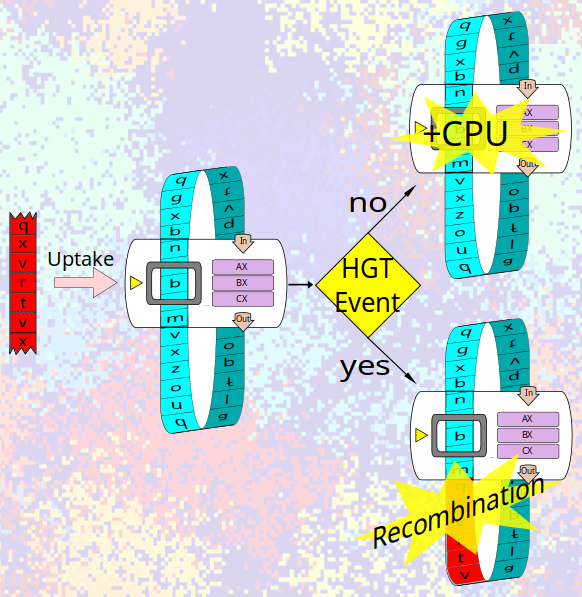
\includegraphics[width=0.7\columnwidth]{figures/hgt_figure.png}
	\caption{\textbf{The HGT process}. Organisms can execute instructions that trigger uptake from the environment. When uptake occurs, there is an experimenter-defined chance that either it will yield a boost to speed of execution or, alternatively, that the fragment will be integrated into the genome.
	}\label{fig:hgtprocess}
	\end{center}
	\end{figure}

\subsubsection{Environmental Conditions}
%=environmental rewards
All experiments in this chapter compared outcomes between static environments, and harsh changing environments. In a similar manner to the experiments listed in the previous chapter (Chapter~\ref{chap:ce-adaptation}, Table~\ref{ce-treatments-h}), task rewards in the harsh changing environment switched from a positive to a negative reward. For the HGT experiments, we did not establish a backbone task that was always rewarded. Rather, we divided the Logic-9 environment into two halves, and alternated positive and negative rewards for each task in each set. There are four pairs of tasks of equivalent complexity, and we randomly allocated one from each pair to an experimental group. We also assigned \texttt{EQU}, which is the most complex task, and has no equivalent, to a random group. Thus, for the first phase of the cycle, we punished the \texttt{NOT}, \texttt{AND}, \texttt{OR}, \texttt{NOR}, and \texttt{EQU} instructions at $-2^1$, $-2^2$, $-2^3$, $-2^4$, and $-2^5$ respectively, while rewarding \texttt{NAND}, \texttt{ORN}, \texttt{ANDN}, and \texttt{XOR} at $2^1$, $2^2$, $2^3$, and $2^4$. In the second phase of the cycle, these rewards flipped, such that we rewarded \texttt{NOT}, \texttt{AND}, \texttt{OR}, \texttt{NOR}, and \texttt{EQU}, and punished \texttt{NAND}, \texttt{ORN}, \texttt{ANDN}, and \texttt{XOR} (See Table~\ref{hgt-treatments-logic9}).

	\begin{table}[]
	\centering
	\caption{\textbf{Logic-9 Rewarded Task Groupings}}
	\label{hgt-treatments-logic9-h}

	\begin{tabular}{|c|c|c|c|}
	\hline
	 & \thead{Tasks} & \thead{Reward \\ Phase 1} & \thead{Reward \\ Phase 2} \\\hhline{|=|=|=|=|}
	 Group 1 & \makecell{ \texttt{NOT} \\ \texttt{AND} \\ \texttt{OR} \\ \texttt{NOR} \\ \texttt{EQU} } & \makecell{ $2^1$ \\ $2^2$ \\ $2^3$ \\ $2^4$ \\ $2^5$ } & \makecell{ $-2^{1}$ \\ $-2^{2}$ \\ $-2^{3}$ \\ $-2^{4}$ \\ $-2^{5}$ } \\\hline
	 Group 2 & \makecell{ \texttt{NAND} \\ \texttt{ORN} \\ \texttt{ANDN} \\ \texttt{XOR} } & \makecell{ $-2^{1}$ \\ $-2^{2}$ \\ $-2^{3}$ \\ $-2^{4}$ } & \makecell{ $2^1$ \\ $2^2$ \\ $2^3$ \\ $2^4$ } \\\hline
	\end{tabular} 

	\begin{flushleft}Logic-9 tasks were divided into to groups, with one task from each pair of tasks of equivalent complexity assigned to a group. The \texttt{EQU} task, which has no complexity equivalent, was arbitrarily assigned to the first group. During the first half of a cycle, we rewarded the first group of tasks and punished the second group (see Reward Phase 1). During the second half of the cycle, reversed the pattern, and rewarded the second group, and punished the first group (Reward Phase 2).  
	\end{flushleft}
	\label{hgt-treatments-logic9}
	\end{table}



%=cycle length
Each complete cycle lasted 1000 updates, and the whole experimental run extended for 200,000 updates.
%=static environment
The static environment rewarded executions of all the Logic-9 tasks at their default levels, with no reward switching.

\subsection{Experimental Design}
%\subsubsection{Evolution of HGT - Alternatives to the Grazing Hypothesis}
%=we subject populations for testing the grazing hypothesis
For the treatments corresponding to the first set of hypotheses on the origins of horizontal gene transfer, we subjected four populations of evolving digital organisms with HGT to harsh changing environments (Table~\ref{hgt-treatments-h}), plus a pair of non-HGT control. The treatments correspond to the combination of two factors: static vs changing environment, and grazing bonus vs no bonus.

%=[TABLE - experimental treatments stage 1]

	\begin{table}[]
	\centering
	\caption{\textbf{Experimental Treatments - Evolution of HGT}}
	\label{hgt-treatments-h}

	\begin{tabular}{|c|c|c|c|}
	\hline
	\thead{Treatment} & \thead{Changing \\ Env. \\ Type} & \thead{HGT \\ Action} & \thead{Bonus} \\\hhline{|=|=|=|=|}
	%Control & Static & None & n/a \\\hline
	\makecell{Static Control \\ (no HGT)} & Static & None & n/a \\\hline
	\makecell{CE Control \\ (no HGT)} & Harsh Cyclic & None & n/a \\\hline
	\makecell{HGT \\ B0.0 \\ (Natural Competence \\ No Bonus)} & Static & \makecell{10\% \\ Recombination \\ Probability} & n/a \\\hline
	\makecell{HGT \\ B0.0 \\ CE \\ (Natural Competence \\ No Bonus)} & \makecell{Harsh \\ Cyclic} & \makecell{10\% \\ Recombination \\ Probability} & n/a \\\hline
	\makecell{HGT \\ B0.8 \\ (Natural Competence \\ with Bonus)} & Static & \makecell{10\% \\ Recombination \\ Probability \\ otherwise \\ Bonus \\ Allocation} & \makecell{$2^{0.8}$ per \\ Uptake} \\\hline
	\makecell{HGT \\ B0.8 \\ CE \\ (Natural Competence \\ with Bonus)} & \makecell{Harsh \\ Cyclic} & \makecell{10\% \\ Recombination \\ Probability \\ otherwise \\ Bonus \\ Allocation} & \makecell{$2^{0.8}$ per \\ Uptake} \\\hline
	\end{tabular} 

	\begin{flushleft}Four treatments corresponding to the combination of two factors: Static vs Changing Environment, and Grazing Bonus vs No Grazing Bonus, plus a non-HGT control, where the HGT instruction is inert.  
	\end{flushleft}
	\label{hgt-treatments}
	\end{table}

%=we test for the mechanisms of why CE promotes HGT
For the second set of hypotheses, where we identify the mechanisms that promote the use of HGT, we manipulated the content of the reservoirs to contain fragments drawn from specific phases in the cyclically changing environment, such that fragments either matched or did not match the environment (Table~\ref{hgt-treatments-h-reservoir}). We then measured HGT use, as well as average fitness effects of the HGT mutations, and the fraction of mutations that led to beneficial phenotype switches.

	%=[TABLE - experimental treatments]
	\begin{table}[]
	\centering
	\caption{\textbf{Experimental Treatments - Effects of HGT}}
	\label{hgt-treatments-h-reservoir}

	\begin{tabular}{|c|c|}
	\hline
	\thead{Treatment} & \thead{Fragment\\Source} \\\hhline{|=|=|}
	HGT & organism death \\\hline
	\makecell{Both} & sampled from organisms from both phases \\\hline
	\makecell{OnPhase} & sampled from organisms from the matching phase \\\hline
	\makecell{OffPhase} & sampled from organisms from the non-matching phase \\\hline
	\end{tabular} 

	\begin{flushleft} Four treatments corresponding to the sources of fragments. The first treatment used the default fragment source (dead organisms from the environment). The second treatment sampled a population for organisms corresponding to both phases, and injected those into the reservoirs. The third and fourth treatments sampled the population, but only injected fragments from the matching and non-matching phases, respectively.  
	\end{flushleft}
	\label{hgt-treatments-reservoir}
	\end{table}

\section{Results and Discussion}

Our results, discussed in detail below, show that both an uptake bonus and changing environment promote the use of HGT, and that the increases in uptake are largely additive. Further, we found that while on average, HGT mutations are neutral, that the majority of the benefits conveyed by HGT in changing environments come from fragments originating in periods of the cycle where the environment matched the current environment. This result is consistent with the information content of the fragment being valuable. Finally, we find that providing only fragments from the matching cycle elevates uptake rates significantly.

%\subsection{Alternatives to the Grazing Hypothesis}
\subsection{Changing environments elevate HGT use}
%Measured HGT fragment uptake in four conditions - 0Static, BStatic, 0CE, BCE.
%* No bonus, static - uptake remains low
%* Bonus, static - uptake increases
%* No bonus, CE - uptake higher than no bonus static
%* Bonus, CE - uptake higher than either BonusStatic or NoBonusCE

%=measured fragment uptake, results summary
We measured HGT fragment uptake in four conditions (see Table~\ref{hgt-treatments-h}), plus of pair of non-HGT controls. Without a bonus, in a static environment, fragment uptake was depressed to a low level as compared to the rate of the non-HGT control, where the \texttt{HGT-Uptake} instruction does nothing (Wilcoxon Rank-Sum Test: Z = 9.74, p $<<$ 0.0001). This result is consistent with HGT in a static environment being largely deleterious (Figure~\ref{fig:hgt_fragment_uptake}). However, in a no-bonus harsh changing environment, fragment uptake was elevated compared to the static environment (Wilcoxon Rank Sum-Test: Z = -8.44, p $<<$ 0.0001). This shows that in the context of a harsh changing environment, the integration of new genetic material is more beneficial than in the static environment. We also found that, regardless of whether the environment is static or changing, when a bonus to fragment uptake was provided (analogous to the nutritive benefit granted by natural competence in biological organisms), fragment uptake also increased (Wilcoxon Rank Sum Test: Z = -8.44, and -7.47, p $<<$ 0.0001). 

	\begin{figure}[h!]
	\begin{center}
	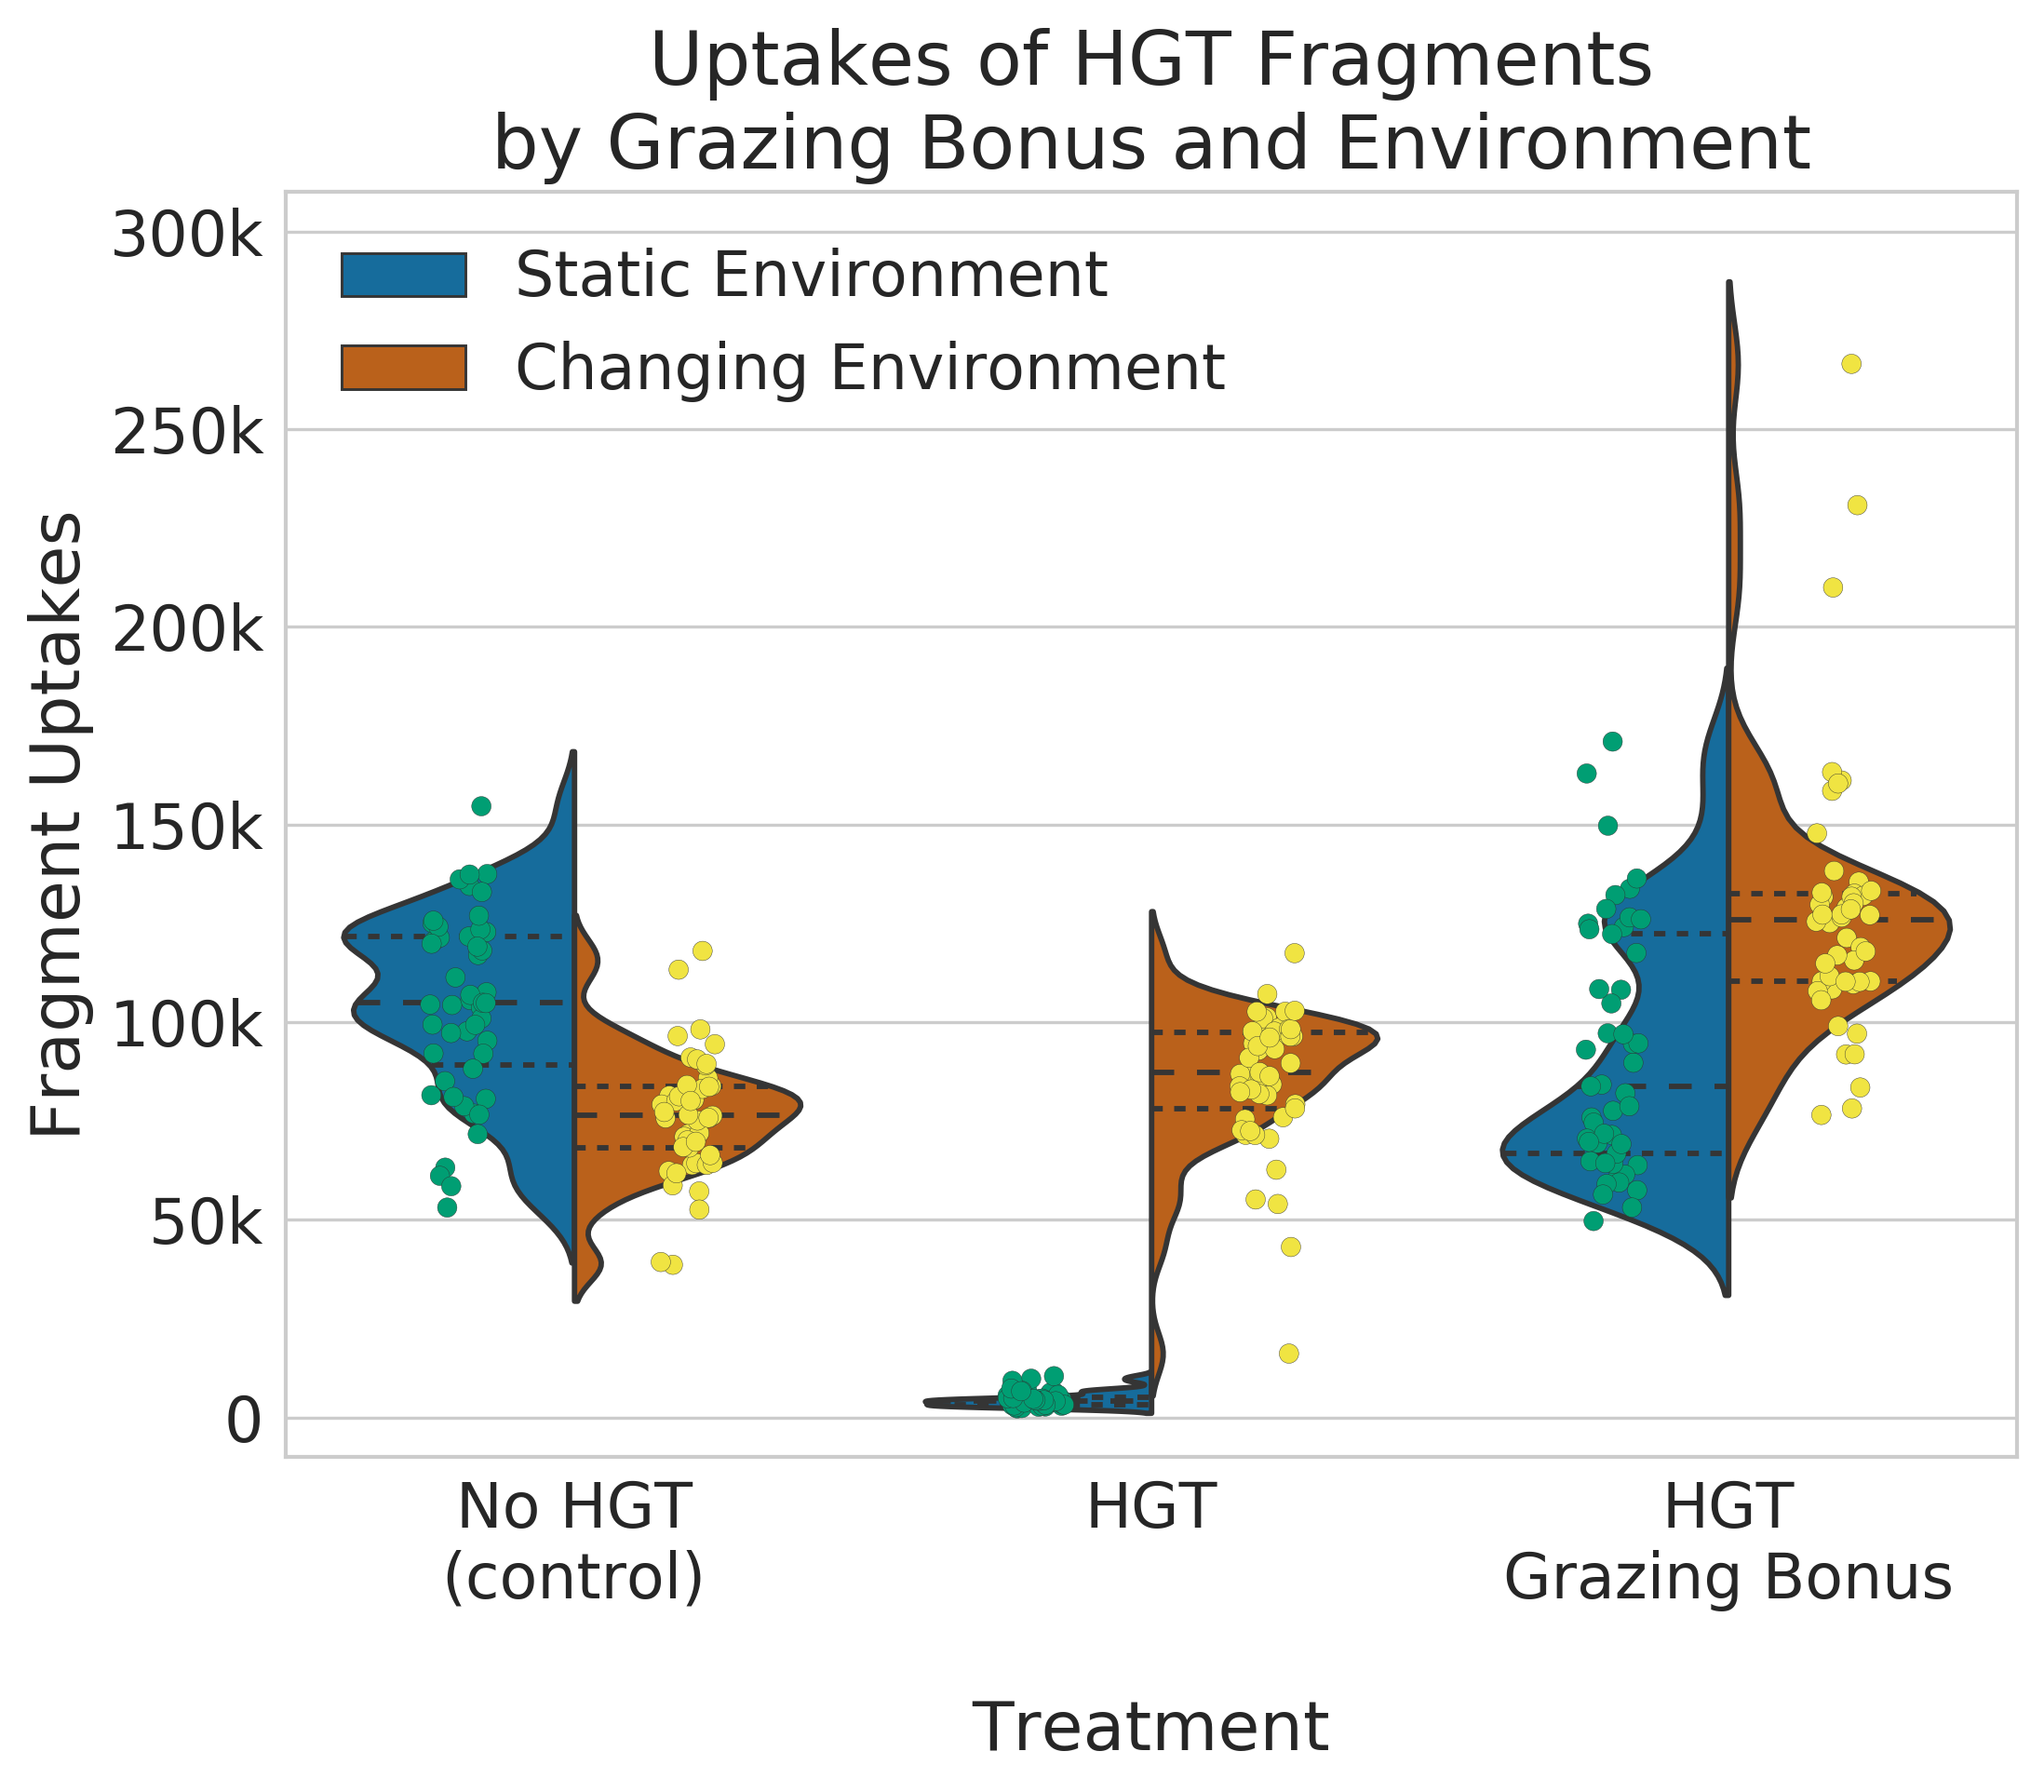
\includegraphics[width=0.75\columnwidth]{figures/hgt_fragment_uptake.png}
	\caption{ \textbf{Number of HGT fragment uptakes} in static and changing environments, without a grazing bonus, with a grazing bonus, and a no HGT control, where the \texttt{HGT-Uptake} instruction is inert. HGT uptake increased in response to a changing environment, and also in response to a grazing bonus. Both the grazing environment and a changing environment resulted in an even larger increase of fragment uptakes than either the changing environment, or the bonus alone (Wilcoxon Rank Sum Test: Z = -4.93 and -7.47 respectively, p $<<$ 0.0001).
	%
	}\label{fig:hgt_fragment_uptake}
	\end{center}
	\end{figure}

%=measured fragment uptake wrl to bonus
In order to investigate the relationship between the effects granted by a nutritive bonus and the benefit of fragment recombination in a changing environment, we selected a bonus level that increased fragment uptake in a static environment to a level comparable to the increase seen in changing environments without a bonus (for more details of this bonus selection, please see Appendix~\ref{appendix:hgt_sweep}). We then combined these factors, giving a bonus plus a changing environment. We saw that the resulting uptake level increased largely additively. This result suggests that the benefits granted by a grazing bonus are generally independent of the benefits conveyed by integrating new genetic material. 
% MJW: The preceding paragraph reads like methods, no?
%@RCK: Eh. I don't know. It's what we measured. Yes, we did a specific experiment, so that should be documented in methods. But I don't mind explaining the measure here.

%=conclusion sentence - hgt is promoted by HGT
Thus, not only is HGT evolution possible absent a bonus, the benefit stacks with that of a grazing bonus, proving a more likely scenario by which HGT might evolve. %bleh


\subsection{HGT derives most benefit from on-cycle fragments, but not all}
%=understanding why HGT is used
\subsubsection{Fitness Effects}
In order to understand the basis of the beneficial nature of HGT in changing environments, we measured the fitness effect of individual fragments on individual organisms within a population.
%=measured fitness effect in normal HGT
We calculated the average fitness effects of fragments of the non-replaced HGT control treatment at the end of the last environmental cycle, and generated a distribution of fragments, and sorted the fragments by age and fitness-effect (Figures~\ref{fig:fitness_effect_heatmap}). We observe a clear pattern of more beneficial fitness effects from fragments of organisms originating in the matching cycle phase. 
% MJW: Have we done this for only one replicate?
%@RCK: yes. It's an example of what they look like. Maybe we don't care that they look this way, but I like the figure :P
%@RCK: Actually, no, this is an aggregation of all replicates, but due to the nature of the analysis, which is an enumeration, there's no averaging or sampling here.

	\begin{figure}[h!]
	\begin{center}
	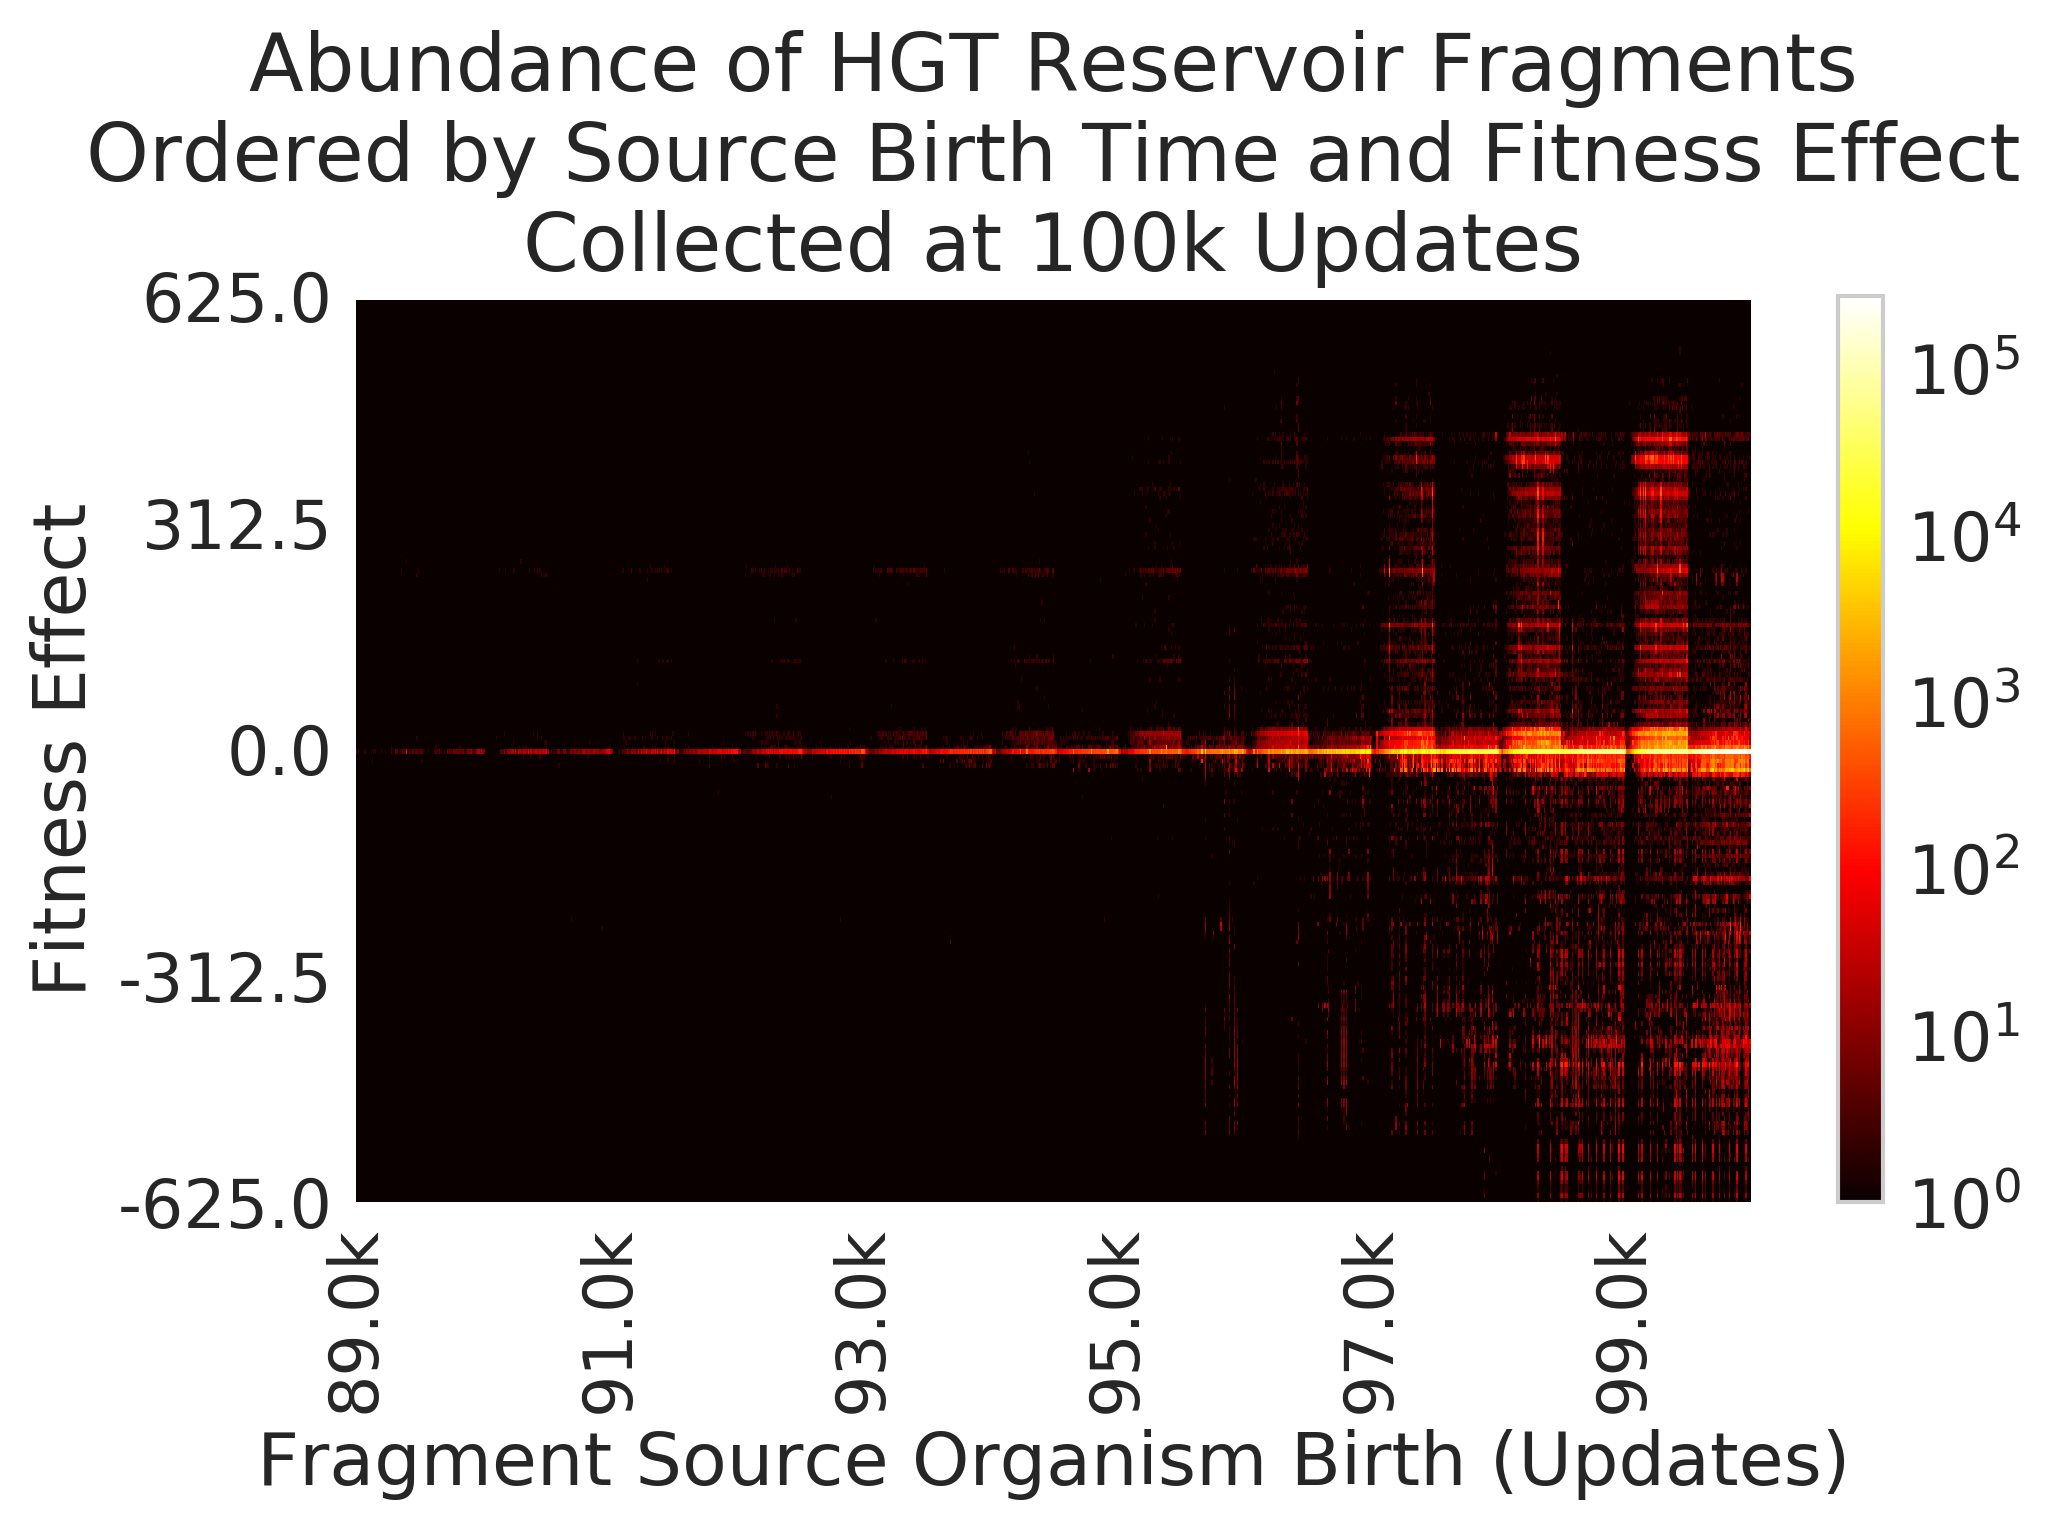
\includegraphics[width=0.75\columnwidth]{figures/fitness_effect_heatmap.png}
	\caption{\textbf{Origin and fitness effect distributions of HGT fragments}, sampled midway through the experiment at 100,000 updates, and aggregated across all replicates. We applied each fragment in each cell's reservoir, one at a time, to the organism in the cell, then recorded the fitness effect. The x-axis is the birth update of fragment's original donor organism. The y-axis is a fragment's fitness effect. The color of each point represents the number of fragments that originate in that birth update a given fitness value. Hotter values indicate more fragments from that time origin at that fitness effect. Most fragments with a positive fitness effect (the upper half of the figure) appear in bands that correspond with the matching phase of an earlier cycle. 
	}\label{fig:fitness_effect_heatmap}
	\end{center}
	\end{figure}


%=manipuated reservoir to match or not match phase - measured effects 
To quantify this observation, we performed experiments where we replaced the fragments in the reservoir with fragments originating in the matching phase, the off-phase, and mixture of both phases as a control. We measured the mean and median fitness effects of fragments in these treatments (Figure~\ref{fig:fitness_effect_by_cycle_phase_source}). We found that HGT mutations were, on average, neutral, or nearly neutral in all the treatments. Both the non-replaced control (Mdn = 0.0, 95\% CI [0, 0]) and the replaced-"both" treatment (Mdn = -0.008, 95\% CI [-0.009, -0.008]) were neutral or nearly neutral. The median fitness effect in the "on-phase" treatment was mildly deleterious (Mdn = -0.054, 95\% CI [-0.055, -0.052]), while the mean was more strongly beneficial (M = 1.19, SD = 19.7). In contrast, in the "off-phase" treatment, the median fitness effect was, again, mildly deleterious (Mdn = -0.0005, 95\% CI [-0.0006, -0.0004]), but with a much more deleterious mean (M = -23.06, SD = 101.8). This suggests that while, on average, HGT mutations remain nearly neutral, a few fragments from the matching phase were strongly beneficial, while the opposite was the case for the non-matching phase.

	\begin{figure}[h!]
	\begin{center}
	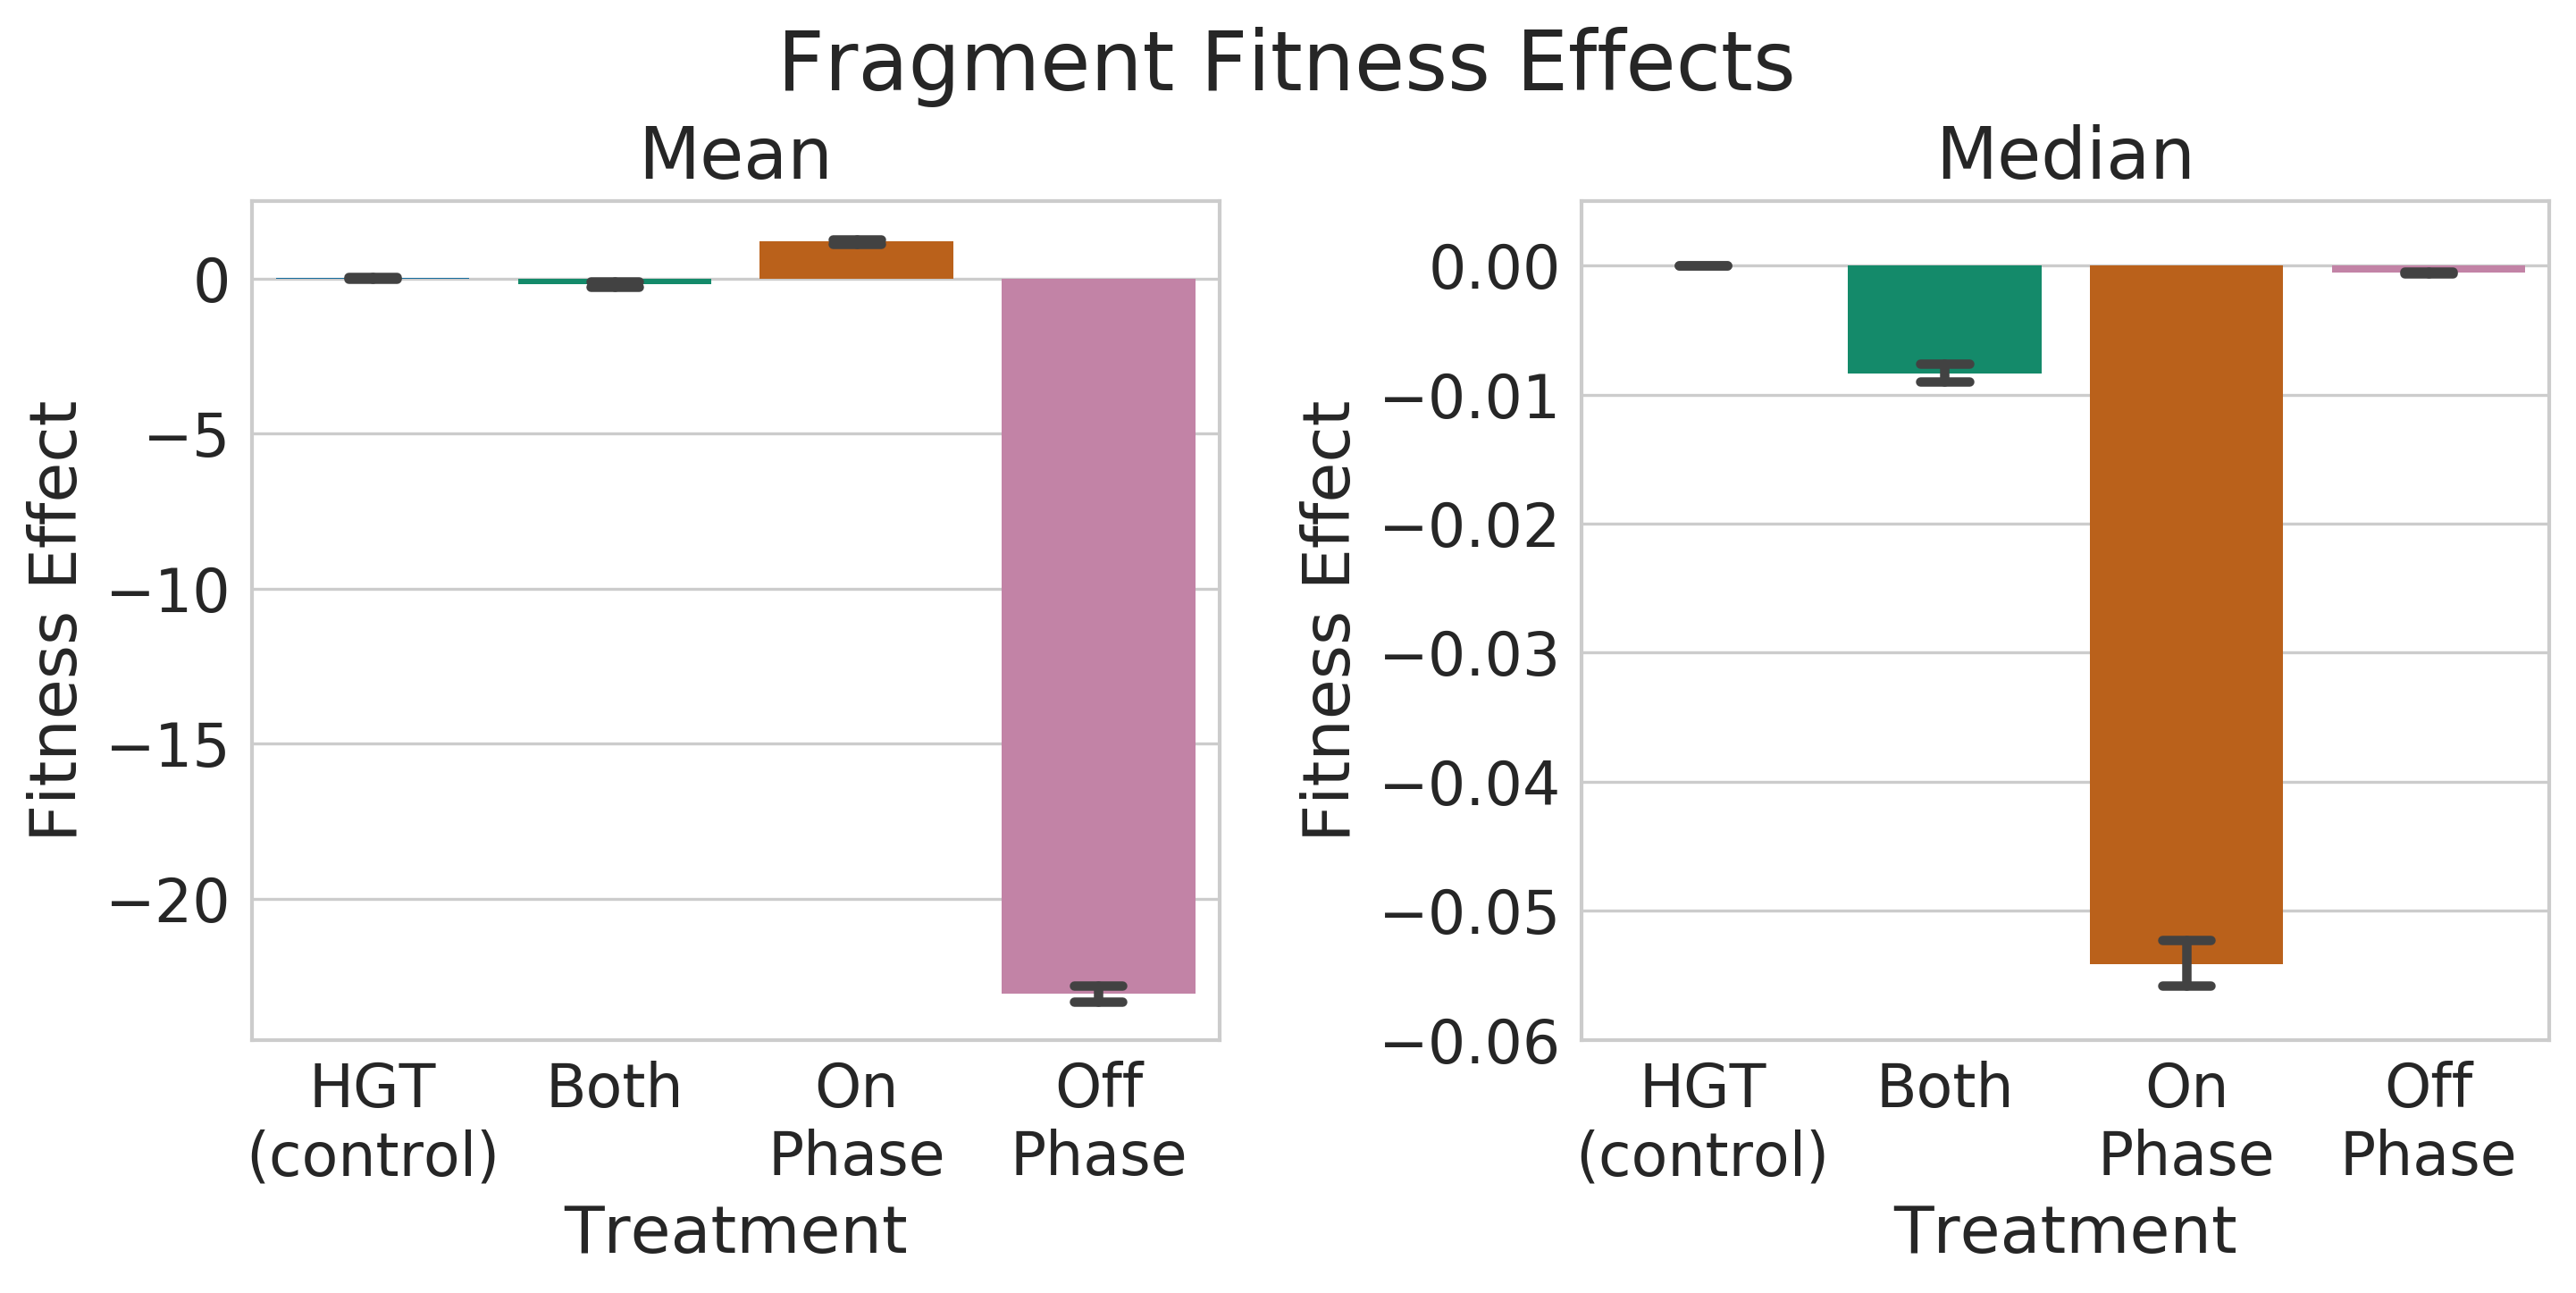
\includegraphics[width=0.95\columnwidth]{figures/fitness_effect_by_cycle_phase_source.png}
	\caption{\textbf{Mean and median fitness effects of fragments} in reservoirs, with 95\% confidence intervals. Fragments in reservoirs are replaced by fragments based on the origin of donor organism. For the On-Phase treatment, We only permitted fragments in reservoirs that originated in a matching phase of the current cycle. For the Off-Phase treatment, we only permitted fragments from non-matching phases. Plus two controls: first, where no filtration takes place, and "Both" where fragments are injected from a mixed set of origins. The Off-Phase treatment had a significantly lower fitness effect than either of the controls (Wilcoxon Rank-Sum Test: Z = 143 and 31 respectively, p $<<$ 0.001), while the On-Phase treatment had a significantly better fitness effect (Wilcoxon Rank-Sum Test: Z = 105 and 3 respectively, p $<$ 0.002). 
	}\label{fig:fitness_effect_by_cycle_phase_source}
	\end{center}
	\end{figure}

\subsubsection{Beneficial Phenotype Switching}
%=measured phenotypic change
In our environments, mutations that convey phenotypic change should have the largest impact. Specifically, the largest fitness benefits should occur when a mutation leads to the acquisition of a new rewarded task, or the loss of a punished task.  

	\begin{figure}[h!]
	\begin{center}
	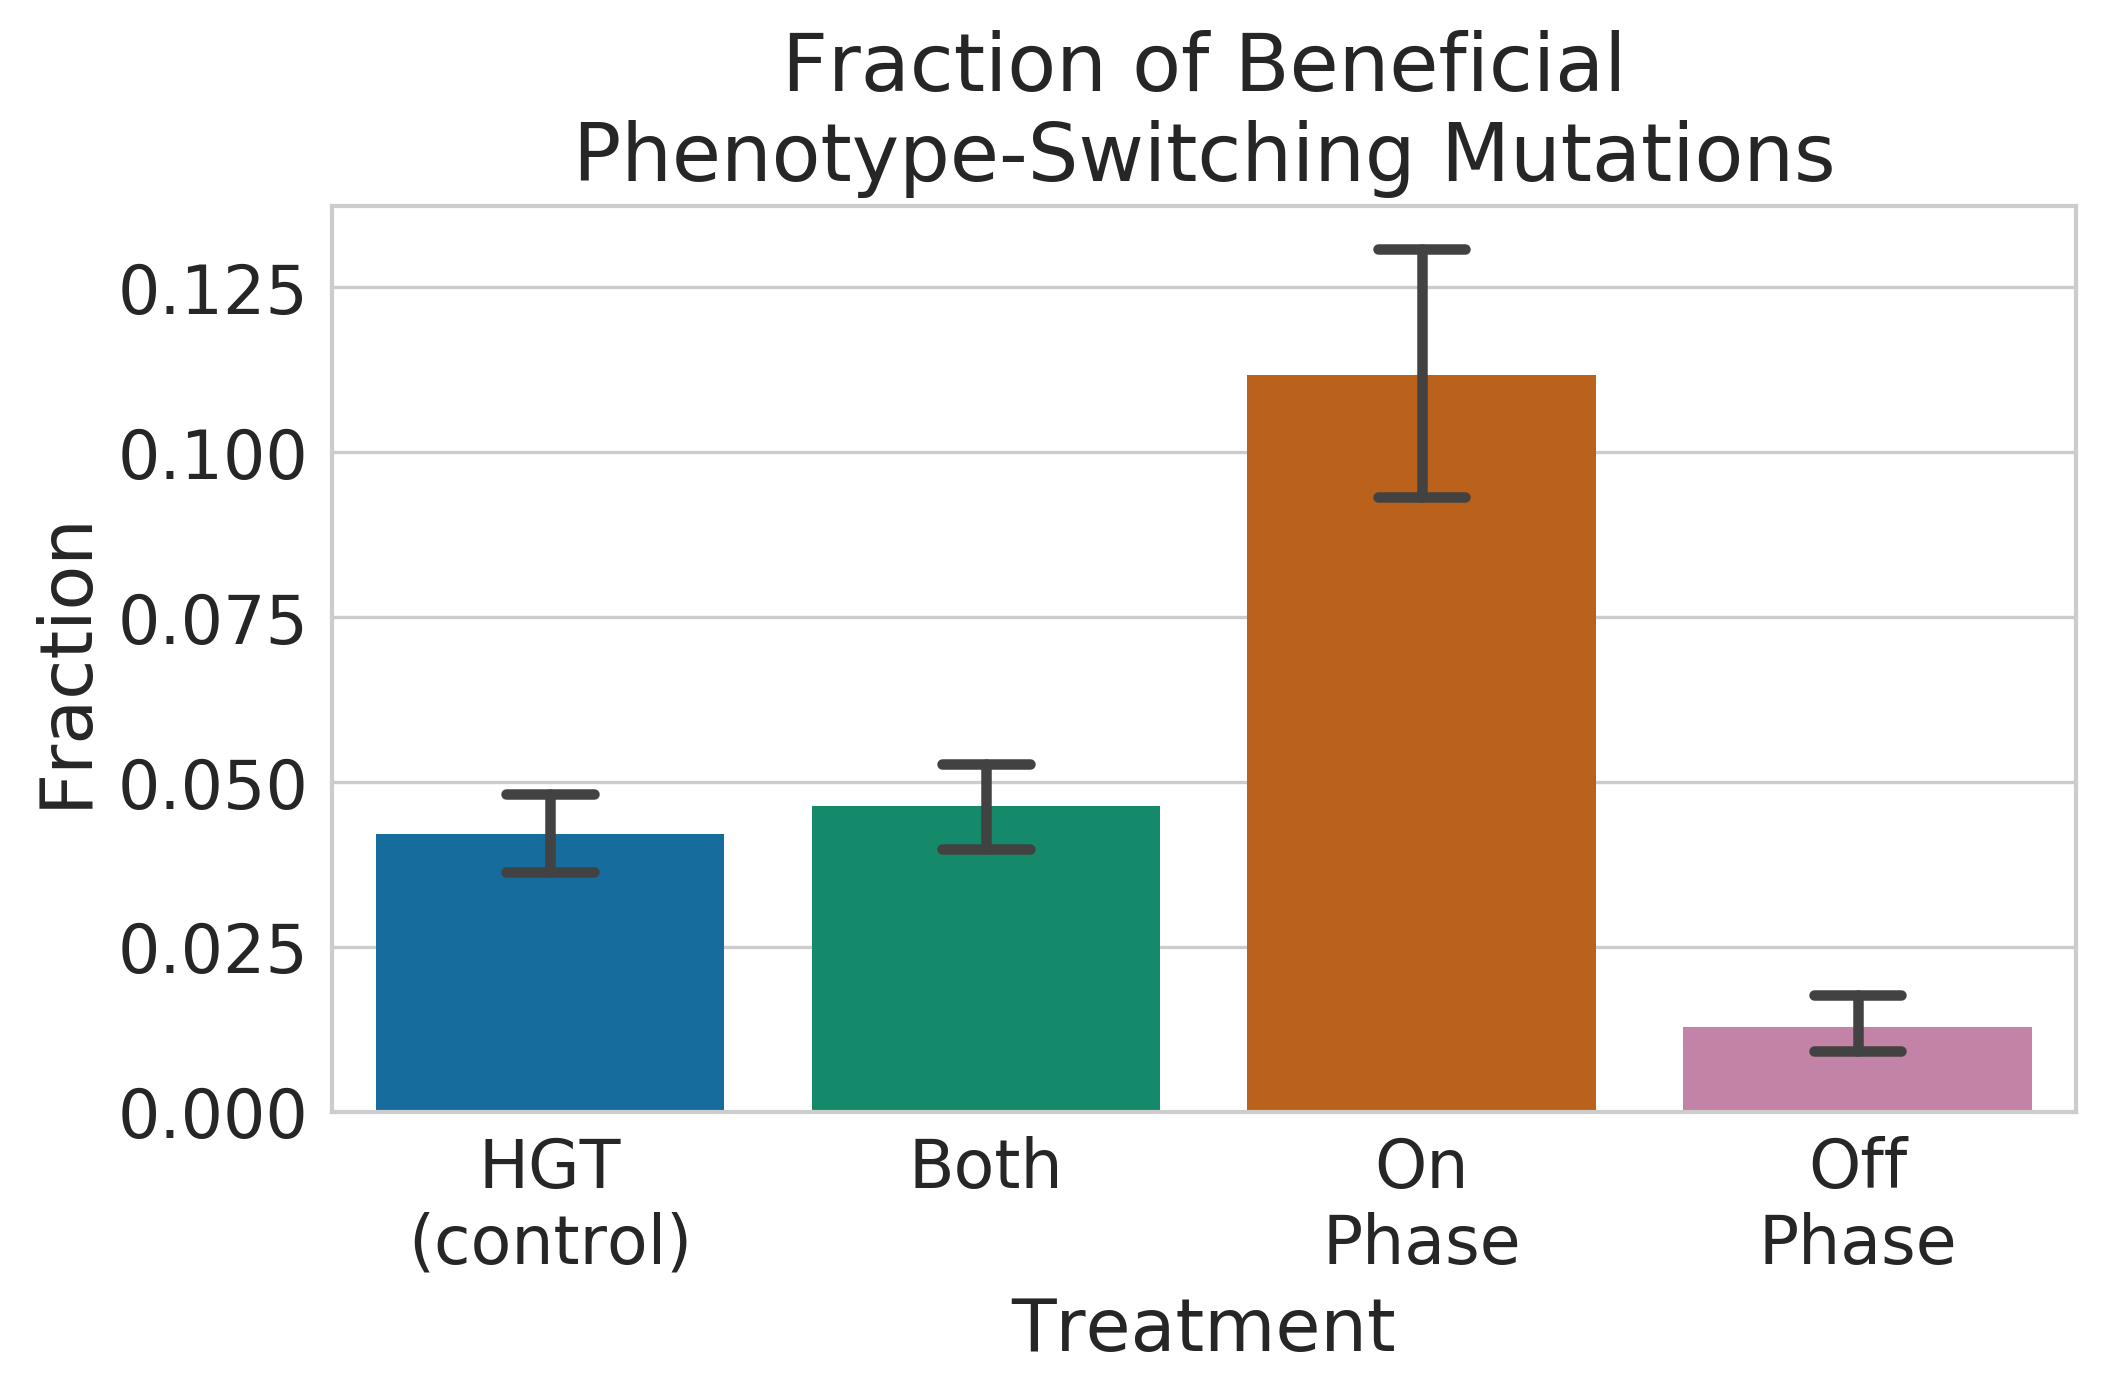
\includegraphics[width=0.75\columnwidth]{figures/beneficial_fraction_by_cycle_phase_source.png}
	\caption{\textbf{Fraction of all fragments that produced a beneficial phenotype changes}, with 95\% confidence intervals. The "On-Phase" treatment had significantly more fragments that convey a beneficial phenotype change than either of the controls (Wilcoxon Rank Sum Test: Z = -6.42 and -6.12 respectively, p $<<$ 0.001), while the "Off-Phase" had significantly fewer (Wilcoxon Rank-Sum Test: Z = 7.11 and 7.35 respectively, p $<<$ 0.001).
	}\label{fig:beneficial_fraction_by_cycle_phase_source}
	\end{center}
	\end{figure}

We quantified the phenotypic effect of each fragment by counting the number of times that fragments produced a beneficial phenotype change, vs all HGT mutations (Figure~\ref{fig:beneficial_fraction_by_cycle_phase_source}). We saw that a significantly larger proportion of fragments in the "on-phase" treatment produced beneficial phenotype changes (Mdn = 0.09, 95\% CI [0.07, 0.11]), as compared to fewer in the normal HGT control (Mdn = 0.03, 95\% CI [0.03, 0.04]) and "both" treatments (Mdn = 0.04, 95\% CI [0.035, 0.05]) (Wilcoxon Rank Sum Test: Z = -6.42 and -6.12 respectively, p $<<$ 0.001). In contrast, we observed virtually no beneficial phenotype changes originating in fragments from the "off-phase" treatment (Mdn = 0.009, 95\% CI [0.006, 0.01]). This result was significantly worse than both the control and the "both" treatments, which produced non-zero beneficial phenotype switches (Wilcoxon Rank-Sum Test: Z = 7.11 and 7.35 respectively, p $<<$ 0.001) 



%=benefit results from matching environment and information conveyed
These results suggest that most direct benefit of using HGT derives from taking up fragments that match the cycle phase of the environment of the affected organism, and thus likely contains information that relates to that environment. %otherwise, it wouldn't matter where the fragment came from
	\begin{figure}[h!]
	\begin{center}
	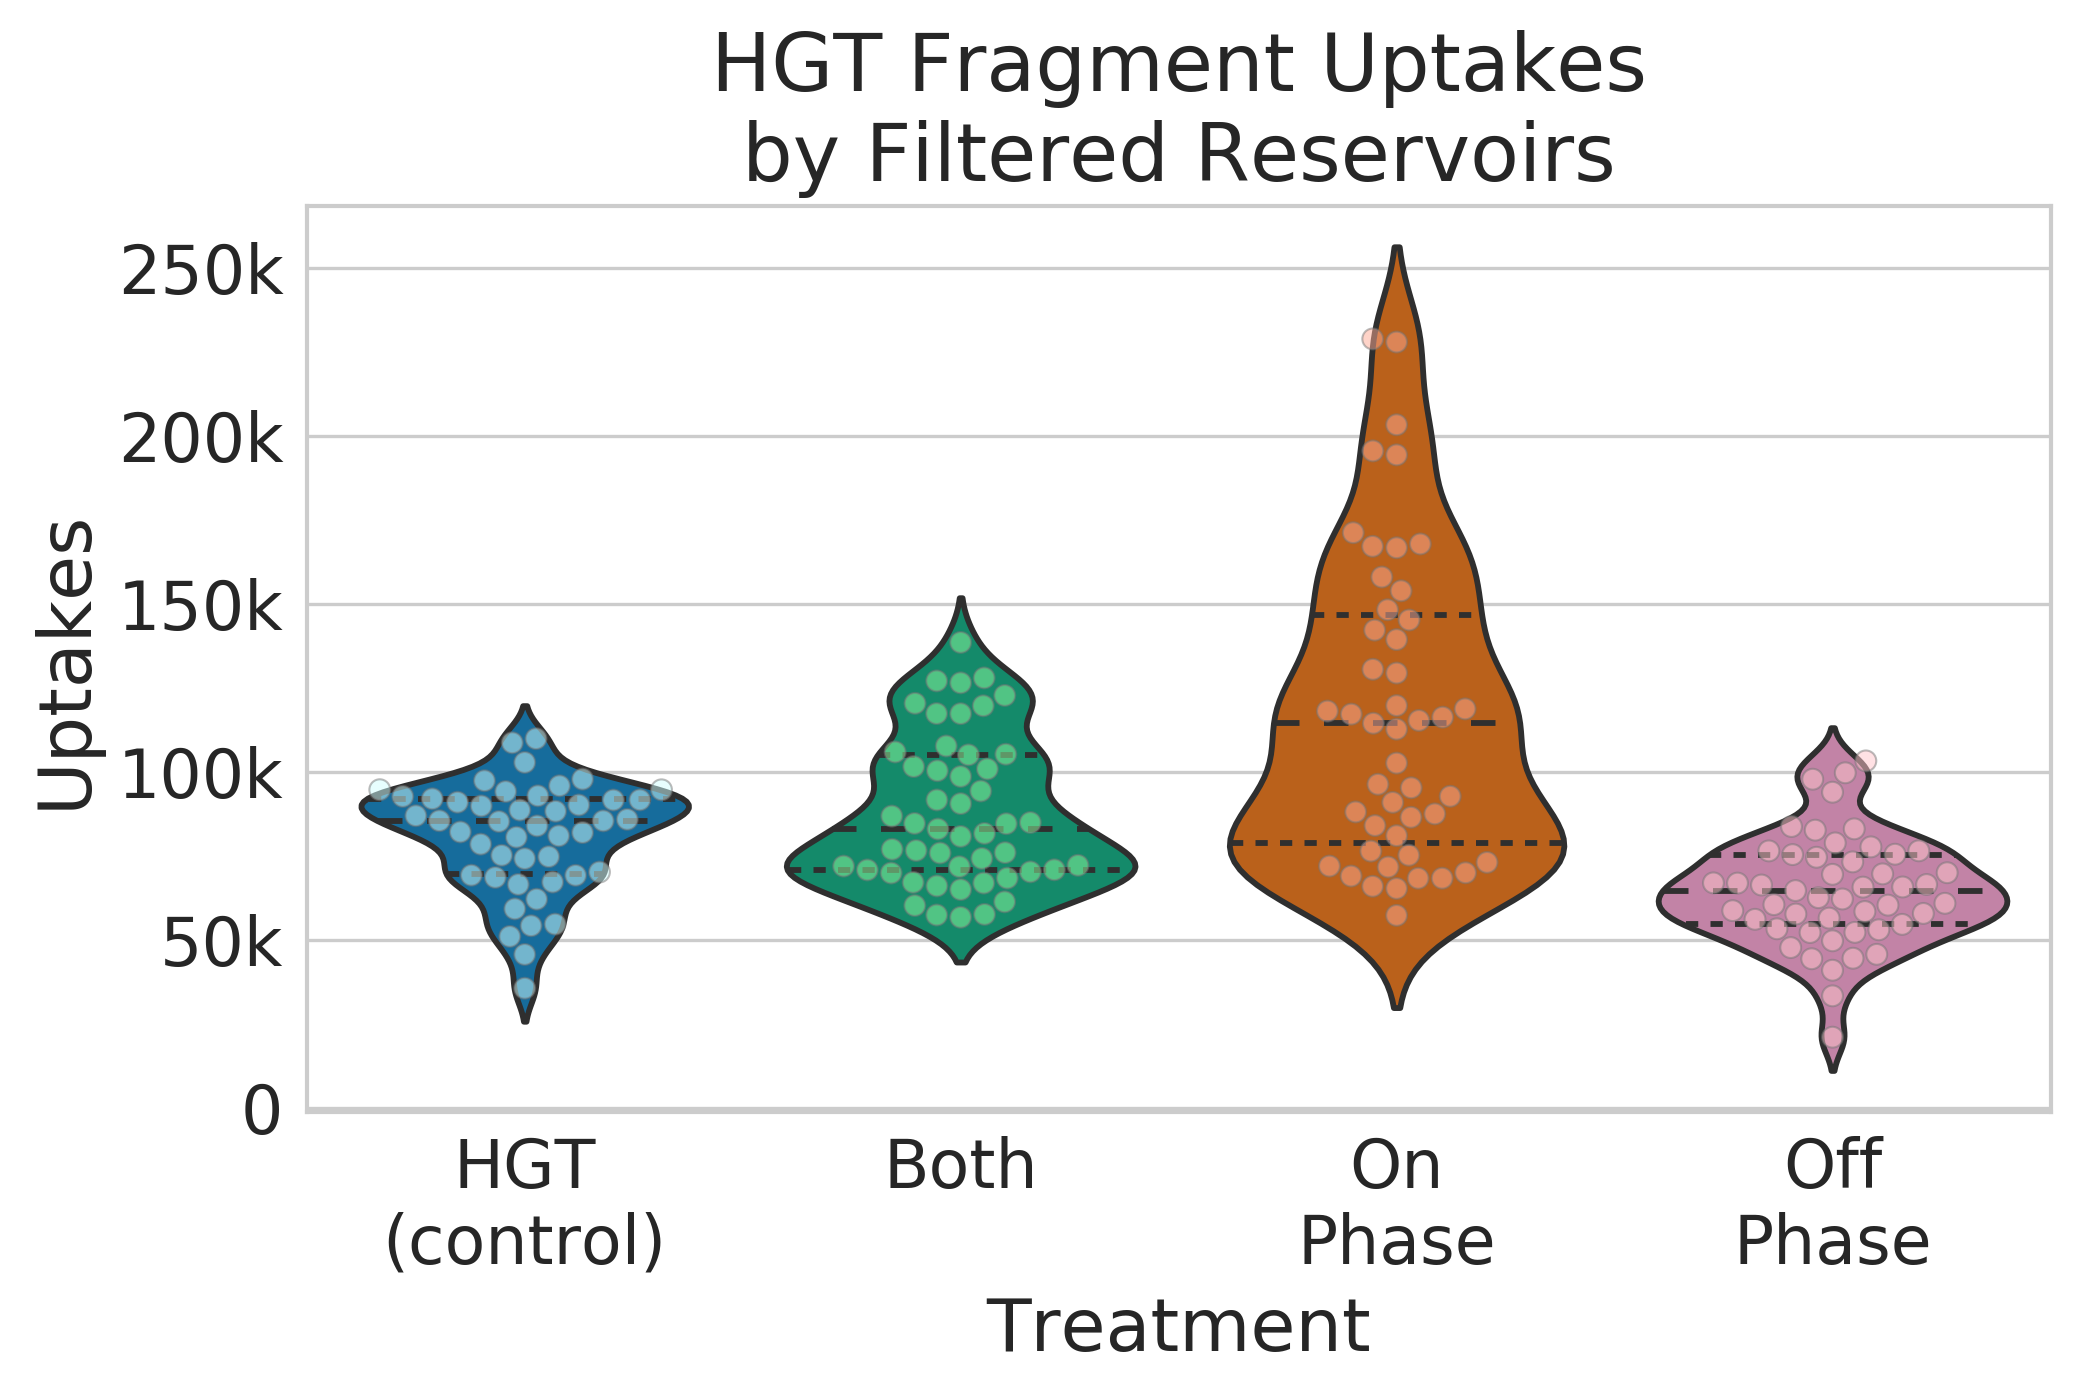
\includegraphics[width=0.75\columnwidth]{figures/hgt_use_by_cycle_phase_source.png}
	\caption{\textbf{Number of uptaken fragments} in the filtered reservoir treatments. The "On-Phase" treatment has a significantly larger number of HGT fragment uptakes, as compared to control, "both", and "off-phase" treatments (Wilcoxon Rank-Sum Test: Z = -3.9**, -3.2*, and -6.5**, respectively, p $<$ 0.002* and p $<<$ 0.001**) This shows that HGT is significantly more beneficial when fragments match the current phase of the cycle. Thus, this suggests that the primary benefit from HGT is not mutational disruption, but the information that fragments convey about the current environment.
	}\label{fig:hgt_use_by_cycle_phase_source}
	\end{center}
	\end{figure}
%=see uptick in use when fragments match phase only.
Further, if fragments from the matching phase are indeed beneficial, we would expect to see an increase in HGT use in those treatments, as compared to those where the fitness effects are mixed or deleterious. And indeed (Figure~\ref{fig:hgt_use_by_cycle_phase_source}), we observed just such an increase. Thus we can conclude that HGT in our changing environments is most beneficial when the fragments in the environment contain information that would be beneficial in that environment. However, even when no such information was available, HGT use was not significantly depressed as compared to the control treatment. This suggests that despite the lack of exclusively matched environmental information, that fragments could still provide some benefit. 

%%%%%%%%%% EXTRA SECTION 
\subsection{Information content of fragments predicts HGT benefit}
\todo[inline, color=magenta]{fill this in - info theory predicts HGT benefit}
%%%%%%%%%%%%%%%%%%%%%%%%%%%%%%%%%%%%%%%

\section{Conclusion}
\todo[inline]{conclusion!}

\section{Acknowledgments}
\todo[inline]{acknowledgements}
\todo[inline]{put in HGT grant \#}

This material is based in part upon work supported by the National Science Foundation under Cooperative Agreement No. DBI-0939454. Any opinions, findings, and conclusions or recommendations expressed in this material are those of the author(s) and do not necessarily reflect the views of the National Science Foundation.
\footnotesize
\bibliographystyle{apalike}
\bibliography{all} 

\end{document}
